% --- SLIDE 1: Titolo (Non mostrata, ma è la tua slide di titolo) ---

% --- SLIDE 2: The Subset Membership Problem ---
\begin{frame}{The Subset Membership Problem}
    \framesubtitle{Querying Collections Efficiently and Compactly}

    Consider a large universe of items $U = \{1, \dots, n\}$, and a specific subset $S \subseteq U$ of $m$ items.

    \begin{alertblock}{Core Task \& Desired Properties}
        \begin{itemize}
            \item Quickly answer: "Is item $x$ in $S$?" (\textbf{Membership Query})
            \item Store $S$ using minimal space (\textbf{Compact Representation})
        \end{itemize}
    \end{alertblock}
    \pause % Pausa prima del ponte a Shannon

    To understand "minimal space", we turn to Information Theory.
    \textit{What is the least number of bits needed to uniquely identify $S$?}
    \pause
    \begin{definition}[Shannon Entropy $H(X)$]
        The average uncertainty, or information content, per symbol of source $X$:
        \[ H(X) = E_{P_X}[-\log_2 P_X(x)] = -\sum_{x \in \mathcal{X}} P_X(x) \log_2 P_X(x) \quad [\text{bits/symbol}] \]
    \end{definition}
\end{frame}

% --- SLIDE 3: Information-Theoretic Limits for Subsets ---
\begin{frame}{Information-Theoretic Limits for Subsets}
    \framesubtitle{From General Entropy to Specific Subsets}
    We usually don't know the true source $P_X$. We only have the data sequence $S$.
    \pause
    \begin{definition}[Zero-Order Empirical Entropy $\mathcal{H}_0(S)$]
        Information content of sequence $S$ based on its symbol counts ($n_s$):
        \[ \mathcal{H}_0(S) = \sum_{s \in \Sigma} \frac{n_s}{n} \log_2 \frac{n}{n_s} \quad [\text{bits/symbol}] \]
        \vspace{-0.2em}
        Uses observed frequencies $\frac{n_s}{n}$ instead of unknown $P_X(x)$.
    \end{definition}

    \pause % Pausa 2
    For our subset $S$ of $m$ items from $n$:
    \begin{itemize}
        \item There are $\binom{n}{m}$ such distinct subsets.
        \item To uniquely identify one, we need at least $\lceil \log_2 \binom{n}{m} \rceil$ bits. This is the \alert{information content} of specifying the subset.
    \end{itemize}

\end{frame}

% --- SLIDE 4: Bitvectors: Querying the Implicit Representation ---
\begin{frame}{Bitvectors: Querying the Implicit Representation}
    \framesubtitle{From Compact Storage to Element Access}

    We can represent our subset $S$ as a \textbf{bitvector} $B[1..n]$ ($B[i]=1 \iff i \in S$). We are \textbf{encoding the choice of $m$ positions for the '1's}, allowing us to store $B$ using $\approx \lceil \log_2 \binom{n}{m} \rceil$ bits (i.e., $\approx n \mathcal{H}_0(B)$ bits). \textit{This means $B$ is not stored as an explicit array of $n$ bits.}

    % Immagine: gestita con \only per cambiare con le pause del testo
    \begin{figure}[htbp]
        \centering
        \only<1-3>{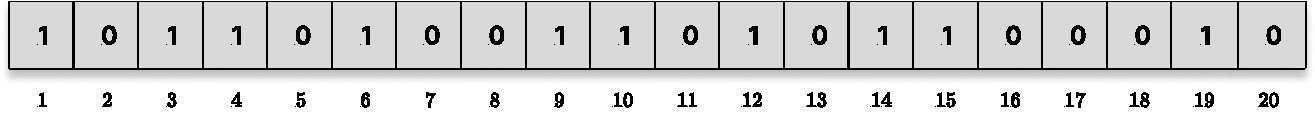
\includegraphics[width=0.95\textwidth]{assets/rank_select_1.pdf}} % Stati 1, 2, 3
        \only<4-5>{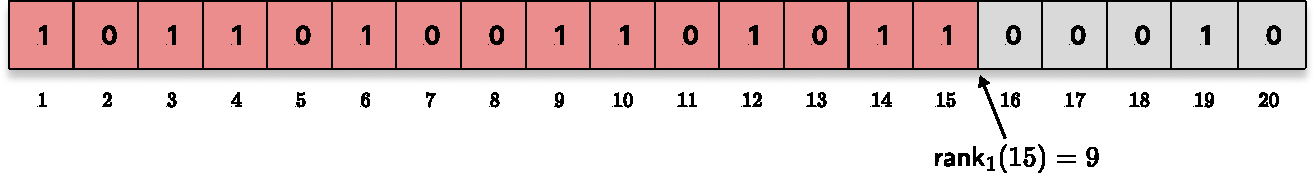
\includegraphics[width=0.95\textwidth]{assets/rank_select_2.pdf}}   % Stati 4, 5
        \only<6->{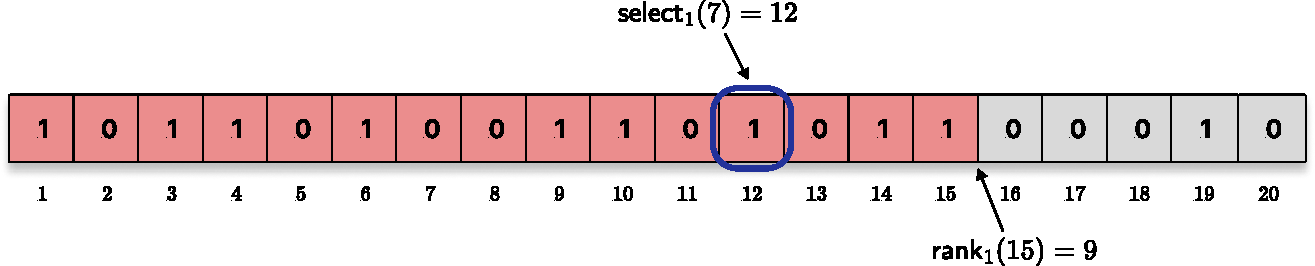
\includegraphics[width=0.95\textwidth]{assets/rank_select_3.pdf}}  % Stato 6 in poi
        \vspace{-0.5em} % Leggero aggiustamento verticale se necessario dopo l'immagine
    \end{figure}

    \pause % STATO 1 -> STATO 2 (appare la domanda)

    \uncover<2->{If $B$ is not explicit, how do we access $B[i]$? We use two foundational queries:}

    \pause % STATO 2 -> STATO 3 (appare def. rank)

    \begin{columns}[T, totalwidth=\textwidth] % Le colonne esistono, ma il contenuto appare in fasi
        \begin{column}{0.52\textwidth}
            \uncover<7->{ % Il blocco "Access Queries" appare per ultimo (STATO 7)
                \begin{block}{\textsf{Access} Queries}
                    $B[i] = 1 \iff \textsf{rank}_1(B, i) > \textsf{rank}_1(B, i-1)$
                \end{block}
            }
        \end{column}
        \begin{column}{0.45\textwidth}
            \begin{itemize}
                \item<3-> \textbf{\textsf{rank}}$_b(B, i)$: How many bits $b$ are in the prefix $B[1..i]$?
                    \pause % STATO 3 -> STATO 4 (immagine rank_select_2)
                \item<5-> \textbf{\textsf{select}}$_b(B, j)$: What is the position of the $j$-th occurrence of bit $b$?
                    \pause % STATO 5 -> STATO 6 (immagine rank_select_3)
            \end{itemize}
        \end{column}
    \end{columns}
\end{frame}

% --- SLIDE 5: RRR Structure: The Bitvector Solution ---
\begin{frame}{RRR Structure: The Bitvector Solution}
    \framesubtitle{$n\mathcal{H}_0(B)$ Space \& $O(1)$ Queries}
    % \begin{block}{Succinct Data Structure for Bitvectors}
    \begin{itemize}
        \item \textbf{Goal:} Support $\textsf{rank}$ and $\textsf{select}$ in $O(1)$ time.
        \item \textbf{Space:} Close to the information-theoretic minimum for the bitvector.
    \end{itemize}
    % \end{block}
    \pause
    \begin{theorem}[RRR Structure]
        A bitvector $B[1..n]$ with $m$ set bits can be represented using
        \[ B(n, m) + o(n) + O(\log \log n) \quad \text{bits}, \]
        where $B(n, m) = \lceil \log_2 \binom{n}{m} \rceil \approx n \cdot \mathcal{H}_0(B)$, while supporting \textsf{rank} and \textsf{select} in $O(1)$ time.
    \end{theorem}
    \pause
    \begin{alertblock}{A Cornerstone Result}
        RRR shows that \textbf{optimal space} \emph{and} \textbf{efficient queries} are possible for subsets.
    \end{alertblock}
\end{frame}

% --- SLIDE 6: Why Succinct Data Structures? ---
\begin{frame}{Why Succinct Data Structures?}
    \framesubtitle{The General Challenge \& Goal}

    RRR is a specific solution to a general problem:
    \begin{block}{Massive Data \& Auxiliary Structures Overhead}
        Modern datasets (Science, Web, AI...) are enormous. Complex analysis demands data in RAM, but auxiliary structures (indexes, trees) needed for queries often \textbf{occupy more space than the data itself}.
        $\implies$ Fitting everything in RAM is a major bottleneck.
    \end{block}
    \pause
    \begin{columns}[T]
        \begin{column}<2->{0.45\textwidth}
            \textbf{Classic Trade-off:}
            \begin{itemize}
                \item \textit{Compression:} Minimal space, but slow/no direct queries.
                \item \textit{Traditional Data Structures:} Fast queries, but large space overhead.
            \end{itemize}
        \end{column}
        \begin{column}<3->{0.55\textwidth}
            \begin{alertblock}{The Succinct Goal: Best of Both Worlds}
                Can we achieve \textbf{both}?
                \begin{itemize}
                    \item Space \alert{near information-theoretic minimum}.
                    \item Efficient queries \alert{directly} on compact data.
                \end{itemize}
            \end{alertblock}
        \end{column}
    \end{columns}
\end{frame}

% --- SLIDE 7: Beyond Bits: General Alphabets ---
\begin{frame}{Beyond Bitvectors: General Alphabets}
    \framesubtitle{Wavelet Trees}
    \vspace{-0.2em}
    Consider a sequence $S[1..n]$ over a \textbf{general alphabet} $\Sigma = \{1, \dots, \sigma\}$. How can we answer \emph{succinctly} queries like \textsf{rank}$_c(i)$, \textsf{select}$_c(j)$, and \textsf{access}$(i)$?
    \begin{figure}[hbtp]
        \centering
        \only<2>{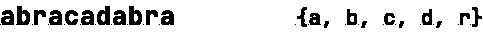
\includegraphics[width=0.6\textwidth]{assets/wt1.pdf}} % Visible only on slide 2
        \only<3>{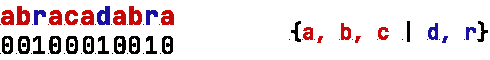
\includegraphics[width=0.7\textwidth]{assets/wt2.pdf}} % Visible only on slide 3
        \only<4>{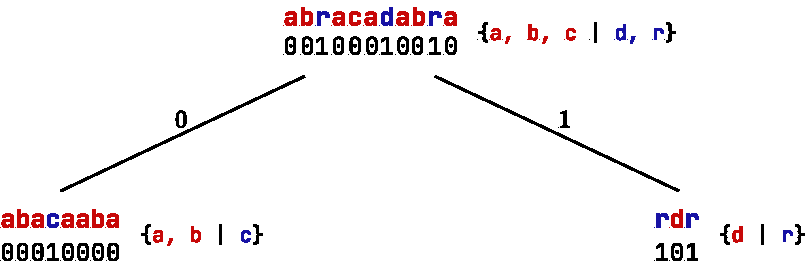
\includegraphics[width=\textwidth]{assets/wt3.pdf}} % Visible only on slide 4
        \only<5>{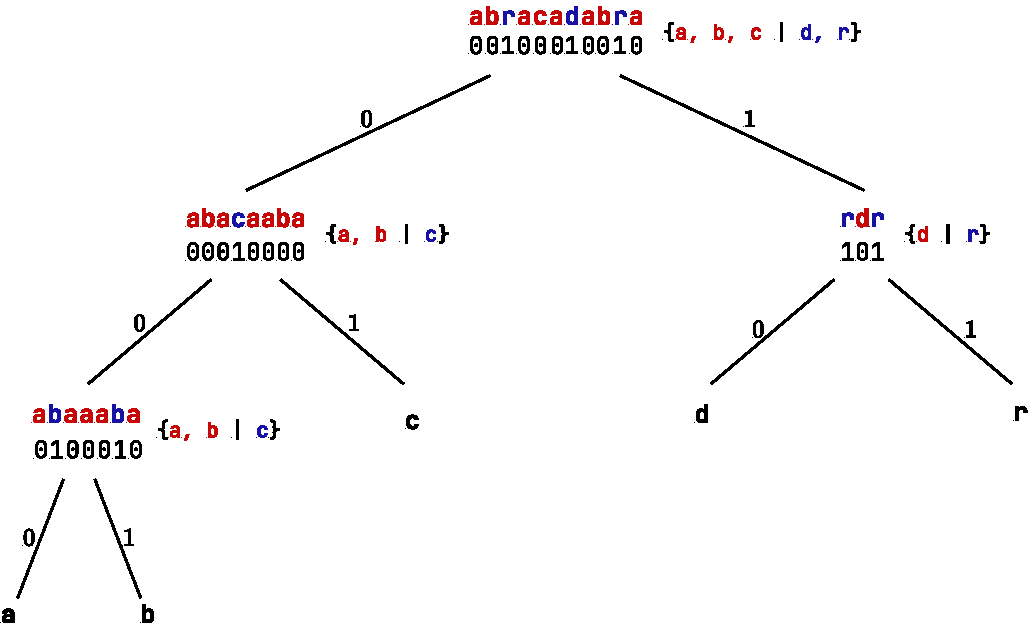
\includegraphics[width=0.7\textwidth]{assets/wt4.pdf}} % Visible ONLY on slide 5
    \end{figure}
    \only<6->{
        \begin{columns}[T] % Align columns at the top
            \begin{column}{0.55\textwidth} % Adjust width as needed
                \centering % Center the image in the column
                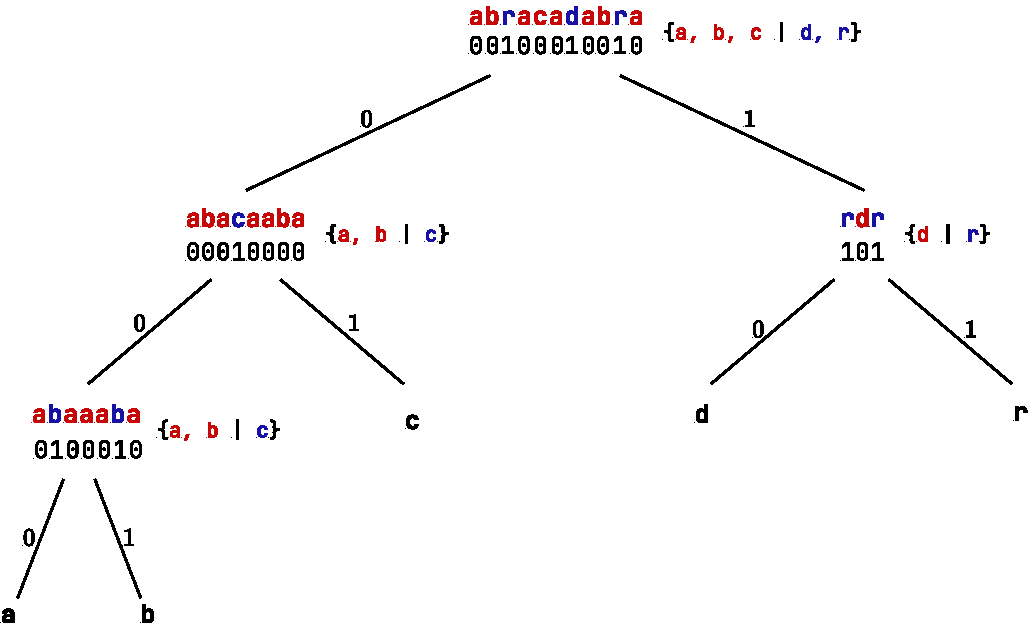
\includegraphics[width=\textwidth]{assets/wt4.pdf}
            \end{column}
            \begin{column}{0.45\textwidth} % Adjust width as needed
                \begin{block}{$\mathcal{H}_0$-Compressed Wavelet Tree} % Ref Thm 3.8 in thesis
                    Using RRR for bitvectors:
                    \begin{itemize}
                        \item \textbf{Space}: $n \mathcal{H}_0(S) + o(n \log \sigma)$ bits.
                        \item \textbf{Query Time}: $O(\log \sigma)$ for \textsf{access}, \textsf{rank}$_c$, \textsf{select}$_c$.
                    \end{itemize}
                    Adapts space to the sequence's zero-order entropy.
                \end{block}
            \end{column}
        \end{columns}
    }
\end{frame}

% --- SLIDE 9: Degenerate Strings ---
\begin{frame}{Representing Sequence Variation: Degenerate Strings}
    \framesubtitle{Definitions and Core Operations}
    \begin{block}{Definition and Rank \& Select Adaptation}
        A \textbf{degenerate string} is a sequence $X = X_1 X_2 \dots X_n$, where each $X_i$ is a \emph{subset} of the alphabet $\Sigma$ with cardinality $\sigma$. We can define the following operations:
        \begin{itemize}
            \item \textsf{subset-rank}$_X(i, c)$: Counts sets $X_k$ ($k \le i$) where $c \in X_k$.
            \item \textsf{subset-select}$_X(j, c)$: Finds index $k$ of the $j$-th set $X_k$ where $c \in X_k$.
        \end{itemize}
    \end{block}
    \begin{figure}[h!] % Nota: [h!] può essere problematico, [htbp] è più sicuro
        \centering
        \begin{tabular}{c@{\hskip 0.5em}c@{\hskip 0.5em}c@{\hskip 0.5em}c@{\hskip 0.5em}c}
            $X = $                                                               & $\Bigg\{\,\begin{matrix}\texttt{A}\\\texttt{C}\\\texttt{G}\end{matrix}\,\Bigg\}$ &
            $\Bigg\{\,\begin{matrix}\texttt{A}\\\texttt{T}\end{matrix}\,\Bigg\}$ &
            $\Bigg\{\,\begin{matrix}\texttt{C}\end{matrix}\,\Bigg\}$             &
            $\Bigg\{\,\begin{matrix}\texttt{T}\\\texttt{G}\end{matrix}\,\Bigg\}$                                                                                                            \\
                                                                                 & $X_1$                                                                            & $X_2$ & $X_3$ & $X_4$
        \end{tabular}
        \uncover<2->{\qquad
            \begin{tabular}{c@{\hskip 0.5em}c@{\hskip 0.5em}c@{\hskip 0.5em}c@{\hskip 0.5em}c@{\hskip 0.5em}c}
                $S =$  & \texttt{ACG} & \texttt{AT} & \texttt{C} & \texttt{TG} &            \\
                $R = $ & \texttt{100} & \texttt{10} & \texttt{1} & \texttt{10} & \texttt{1} \\
                       & $S_1$        & $S_2$       & $S_3$      & $S_4$
            \end{tabular}
        }
    \end{figure}
    % --- Paragrafo Riscritto ---
    \uncover<3->{% Potrebbe essere utile per far apparire il testo solo al terzo step
        To compute \textsf{subset-rank}$_X(i, c)$: Let $p$ be the end position in $S$ for prefix $X_1..X_i$, found using $\textsf{select}_1(R, i+1)$. The result is $\textsf{rank}_c(S, p)$.
    }
\end{frame}
